\documentclass[11pt,a4paper]{article}

\usepackage[T1]{fontenc}
\usepackage{lmodern}
\usepackage[utf8]{inputenc}
\usepackage[margin=2.5cm]{geometry}
\usepackage{amsmath,amssymb,amsthm}
\usepackage{booktabs,tabularx,threeparttable}
\usepackage{graphicx}
\usepackage[font=small,labelfont=bf]{caption}
\usepackage[round,authoryear]{natbib}
\usepackage{microtype}
\usepackage{xcolor}
\usepackage[colorlinks=true,linkcolor=blue!50!black,citecolor=blue!50!black,urlcolor=blue!50!black]{hyperref}
\hypersetup{pdftitle={Backtest Overfitting Statistics under Serial Dependence},pdfauthor={Mayank Khandelwal}}
\usepackage{xurl}
\usepackage[section]{placeins}
\usepackage{setspace}
\setstretch{1.08}

\newcommand{\SR}{\mathrm{SR}}
\newcommand{\hSR}{\widehat{\mathrm{SR}}}
\newcommand{\E}{\mathbb{E}}
\newcommand{\Var}{\operatorname{Var}}
\newtheorem{proposition}{Proposition}
\theoremstyle{remark}
\newtheorem{remark}{Remark}

\title{\Large\textbf{Backtest Overfitting Statistics under Serial Dependence}\\[4pt] \large A Computational Replication and Empirical Stress Test}
\author{Mayank Khandelwal\thanks{The code, saved outputs and correction history are in the accompanying repository; Section~\ref{sec:repro} and Appendix~\ref{app:repro} describe what can and cannot be reproduced from a fresh copy. Comments welcome.}}
\date{Working paper, 12 November 2026}

\begin{document}
\maketitle

\begin{abstract}
\noindent
Backtest-validation statistics are often used as fixed hurdles: a probabilistic or deflated Sharpe ratio (PSR, DSR) above 0.95, a probability of backtest overfitting (PBO) below 0.05. We reimplement these statistics, reproduce selected numerical examples from the source papers, and measure their operating characteristics when one idealized assumption fails. With zero true Sharpe, uncorrected PSR(0) rejects 11.85\% [10.47, 13.35] of the time at a nominal 5\% under Gaussian AR(1) dependence with $\phi=0.3$, matching the long-run-variance prediction of 11.37\%; this confirms a known limitation. On block-bootstrapped daily US industry returns with means removed, the error follows each period's dependence in both directions: 8.35\% [7.17, 9.65] for 1971--1998 and 3.85\% [3.05, 4.79] for 1999--2026. The 2014 DSR accepts far fewer than 5\% of zero-skill search winners (0.05\% in an IID search of 100), and more as strategies become correlated. In a search over 93 moving-average rules on the US market factor, the selected rule has DSR 0.998 and PBO 0.208, yet no rule beats buy-and-hold under a paired autocorrelation-robust test (selected rule one-sided $p=0.094$; Hansen's SPA $p=0.50$), and walk-forward re-selection earns a lower Sharpe ratio than the market. Results are conditional on the designs studied; no new statistic is proposed.
\end{abstract}

\noindent\textbf{Keywords:} backtest overfitting; Sharpe ratio; probabilistic Sharpe ratio; deflated Sharpe ratio; CSCV; PBO; multiple testing; serial dependence; replication.\\
\noindent\textbf{JEL:} C12, C15, C22, C58, G11, G17.

\section{Introduction}\label{sec:intro}

A backtest is the output of a search. When many strategy variants are evaluated on the same history and the best is reported, the reported Sharpe ratio is biased upward even if no variant has skill \citep{bailey2014pseudo,harvey2016cross}. A family of statistics was proposed to quantify this effect. The probabilistic Sharpe ratio (PSR) and minimum track record length (MinTRL) attach an asymptotic confidence level to one Sharpe ratio after allowing for skewness and kurtosis \citep{bailey2012frontier}. The deflated Sharpe ratio (DSR) applies PSR against a benchmark equal to the expected maximum Sharpe ratio of $N$ zero-skill trials \citep{bailey2014dsr}. The minimum backtest length (MinBTL) relates the number of trials to the sample length needed before the expected best noise Sharpe falls below a target \citep{bailey2014pseudo}. The probability of backtest overfitting (PBO), estimated by combinatorially symmetric cross-validation (CSCV), measures how often the in-sample winner of a strategy set ranks below the median out of sample \citep{bailey2017pbo}.

The source papers themselves suggest hurdle readings: \citet[p.~10]{bailey2014dsr} read DSR above 0.95 as 95\% confidence in the selected strategy, and \citet[p.~14]{bailey2017pbo} describe PBO at most 0.05 as a customary acceptance rule. Each hurdle inherits assumptions. The PSR variance is derived for independent and identically distributed (IID) returns; the DSR benchmark depends on an estimated number of independent trials; and CSCV's reference value of one half relies on exchangeability. This paper asks two questions.

\begin{enumerate}
\item[\textbf{Q1.}] How reliable are these statistics, as decision rules, when returns are serially dependent, heteroskedastic, heavy tailed, or cross-sectionally correlated, and when the data are real daily returns rather than simulations?
\item[\textbf{Q2.}] Does a historically superior trading rule, selected from a search, survive inference that controls both for the search and for the relevant benchmark?
\end{enumerate}

\noindent We test the following hypotheses, each with a stated null. (H1) Uncorrected PSR(0)$>0.95$ on a zero-Sharpe series rejects at 5\% under each departure from IID Normality. (H2) Its rejection rate under stationary dependence is predicted by the long-run variance factor of the sample mean. (H3) DSR$>0.95$ on the best of $N$ zero-skill trials has a rejection rate near 5\%. (H4) Mean PBO is 1/2 in exchangeable zero-edge sets regardless of the noise process. (H5) The Sharpe ratio of a moving-average rule selected from 93 settings does not exceed that of buy-and-hold. H1 and H3 are hurdle readings rather than claims made by the original authors; Section~\ref{sec:framework} states what the source papers do and do not assert.

\paragraph{Contributions.} We separate what is confirmed from what is new evidence. \emph{Confirmations of known results:} (i)~an independent, test-driven implementation that reproduces the selected numerical examples listed in Table~\ref{tab:replication}, with page-level provenance; (ii)~the over-rejection of PSR under AR(1) dependence, which follows from standard long-run-variance theory \citep{lo2002} and was identified as a defect of the time-series claim in \citet[Remark~3.1]{ledoit2008}. \emph{New quantitative evidence, conditional on the designs studied:} (iii)~the operating characteristics of the 2014 DSR under IID, dependent, heavy-tailed and correlated searches, including its sensitivity to the trial-count convention; (iv)~a demonstration on daily industry returns that PSR's error is period dependent and two directional, with a long-run-variance approximation that matches both periods to within 0.1 percentage points; (v)~a case study in which a high DSR coexists with no evidence of outperforming the market, with the power of the market test (a Normal approximation), a joint SPA data-snooping test and a walk-forward check reported. We claim no new statistic, no first identification of the serial-correlation problem, and no profitable strategy.

\paragraph{Summary of results.} Of the departures studied, only serial correlation materially distorts uncorrected PSR(0); GARCH, Student-$t$ and equicorrelated designs leave its zero-Sharpe rejection rate statistically indistinguishable from 5\%. The distortion is predicted by $\pi(F)=1-\Phi(z_{0.95}/\sqrt{F})$, where $F$ is the long-run variance factor of the sample mean. The 2014 DSR is not a 5\% test under any null studied; its rejection rate is between 0.00\% and 0.70\% except under strong cross-strategy correlation, where it reaches 2.6\% with $N=100$ and 5.05\% with the interpolated effective $N$. Mean PBO stays near its exchangeable reference in every zero-edge design. In the case study, the selected rule's in-sample Sharpe advantage over the market (0.130 per year) is within sampling error, the test has low power against effects of that size, and the advantage does not survive walk-forward re-selection.

\paragraph{Organization.} Section~\ref{sec:lit} reviews related work. Section~\ref{sec:framework} sets out the statistics and the dependence results used. Section~\ref{sec:design} describes the designs and inference conventions, including which analyses were pre-specified. Section~\ref{sec:replication} reports the replication; Section~\ref{sec:results} the empirical results; Section~\ref{sec:robust} robustness checks; Section~\ref{sec:discussion} discusses interpretation; Section~\ref{sec:limits} lists limitations; Section~\ref{sec:conclusion} concludes. Appendices contain derivations, algorithms, extended tables, the correction history and reproducibility details.

\section{Related literature}\label{sec:lit}

\paragraph{Sampling theory of the Sharpe ratio.} \citet{jobson1981} and \citet{memmel2003} give the asymptotic variance of a Sharpe ratio and of the difference of two Sharpe ratios under IID Normal returns. \citet{lo2002} derives standard errors under IID returns and, using the generalized method of moments with a heteroskedasticity- and autocorrelation-consistent (HAC) covariance, under serial dependence; he also shows that annualizing by $\sqrt{q}$ is incorrect when returns are autocorrelated. Mertens (2002), as cited by \citet{bailey2012frontier}, gives the IID non-Normal variance that PSR uses. \citet{christie2005} estimates Sharpe-ratio covariances by GMM with an autocorrelation-consistent weighting matrix, but his closed-form appendix is contemporaneous (lag zero). \citet{opdyke2007} equates that closed form with Mertens' and states that it holds for stationary ergodic returns. \citet[p.~4, p.~8]{bailey2012frontier} cite Opdyke for the statement that their results hold under such conditions. \citet[Remark~3.1]{ledoit2008} note that Opdyke's time-series formulas reduce to the IID formulas and are therefore incorrect for dependent data, and propose HAC and studentized block-bootstrap tests of Sharpe-ratio differences. \citet{pav2021} surveys the area. Our AR(1) result is a numerical instance of this known problem, not a new finding.

\paragraph{Selection and multiple testing.} \citet{white2000} introduced the Reality Check for the best of many forecasting rules against a benchmark, \citet{hansen2005} the test for superior predictive ability (SPA), which reduces the influence of poor rules, and \citet{romano2005} a stepwise procedure that identifies which rules outperform. \citet{sullivan1999} applied the Reality Check to moving-average and other technical rules on US index data, extending \citet{brock1992}; on the Dow Jones index the best rule's superiority survived the Reality Check in 1897--1986 but was not repeated in 1987--1996 \citep[p.~37]{sullivan1999}. Our case study is a small instance of their design applied to the CRSP market factor. \citet{harvey2014evaluating,harvey2015backtesting} and \citet{harvey2016cross} propose multiple-testing haircuts for Sharpe ratios and factor $t$-statistics.

\paragraph{Backtest-overfitting statistics.} \citet{bailey2014pseudo} derive MinBTL from the expected maximum of $N$ standard Normals. \citet{bailey2017pbo} define PBO and estimate it with CSCV. \citet{bailey2014dsr} define the DSR and an interpolation for the effective number of independent trials; \citet{lopezdeprado2018lewis} estimate the effective number of trials by clustering instead.

\paragraph{Later formulations.} \citet{lopezdeprado2026porcu} present the 2014 construction as a location benchmark (DSR-L) within a family that adds scale (DSR-LS) or uses the complete search distribution (DSR-EO), and derive calibration results linking approximation error to false-positive distortion. \citet{lopezdeprado2026lipton} revisit PSR, MinTRL and DSR as reporting standards, and \citet{lopezdeprado2026garch} derive Sharpe-ratio inference under GARCH returns. We examined only the abstracts and metadata of these three papers. Their framework may already explain, and in part correct, the DSR operating characteristics reported in Section~\ref{sec:res:dsr}; our evaluation concerns only the 2014 construction.

\paragraph{Dependence in daily portfolio returns.} Daily portfolio returns show positive autocorrelation that is partly induced by nonsynchronous trading \citep{lo1988,lo1990}. This is relevant to the period effect in Section~\ref{sec:res:real}.

Table~\ref{tab:lit} summarizes how this paper relates to that literature. The column ``novelty limitation'' records why each extension should not be read as more than it is.

\begin{table}[t]
\centering\small
\caption{Position relative to existing work.}\label{tab:lit}
\begin{tabularx}{\textwidth}{@{}>{\raggedright\arraybackslash}p{2.5cm}>{\raggedright\arraybackslash}X>{\raggedright\arraybackslash}X>{\raggedright\arraybackslash}X>{\raggedright\arraybackslash}X@{}}
\toprule
Existing work & Established finding & Our replication & Our extension & Novelty limitation \\
\midrule
Bailey and L\'opez de Prado (2012) & PSR, MinTRL for IID non-Normal returns & All printed examples (Table~\ref{tab:replication}) & PSR rejection rates under 8 departures & GARCH and $t$ cells test only $\SR^\ast=0$ \\
Lo (2002); Ledoit and Wolf (2008) & IID variance invalid under dependence & AR(1) rate matches Eq.~\eqref{eq:ar1rate} & Two-directional, period-dependent error on industry data & Mechanism is textbook long-run variance \\
Bailey and L\'opez de Prado (2014) & DSR, implied $N$ (Eq.~9) & Printed DSR and $\mathrm{SR}_0$ & Null rates under IID, AR, GARCH, $t$, correlation & Later DSR variants (2026) not evaluated \\
Bailey et al.\ (2014, 2017) & MinBTL, PBO via CSCV & Expected max, MinBTL; CSCV counts & PBO under non-IID nulls; one market case & Exchangeable nulls guarantee mean 1/2 \\
White (2000); Hansen (2005); Sullivan et al.\ (1999) & Search-aware benchmark tests; best DJIA rule survives in sample, fails 1987--96 & SPA on 93 rules & Contrast of DSR with benchmark test, power & One market, one rule family \\
\bottomrule
\end{tabularx}
\end{table}

\section{Statistical framework}\label{sec:framework}

\subsection{Notation and the Sharpe estimator}
Let $r_1,\dots,r_T$ be excess returns at a fixed frequency with mean $\mu$, variance $\sigma^2$, skewness $\gamma_3$ and raw kurtosis $\gamma_4$ (Normal: $\gamma_4=3$). The per-period Sharpe ratio and its estimator are
\begin{equation}\label{eq:sr}
\SR=\frac{\mu}{\sigma},\qquad \hSR=\frac{\bar r}{\hat\sigma},\qquad \hat\sigma^2=\frac1T\sum_{t=1}^T(r_t-\bar r)^2 .
\end{equation}
We use the divisor $T$ (our convention, matching the moment code in \citealp[App.~A.4]{bailey2012frontier}). For display, daily values are multiplied by $\sqrt{q}$ with $q=250$ \citep[p.~10]{bailey2014dsr}. Under serial dependence this ``annualized marginal Sharpe'' is not the Sharpe ratio of annual summed returns; we use it only as a display scale.

Under IID returns with finite fourth moment, the delta method gives
\begin{equation}\label{eq:mertens}
\sqrt{T}\,(\hSR-\SR)\ \xrightarrow{d}\ \mathcal N\!\left(0,\;1-\gamma_3\SR+\tfrac{\gamma_4-1}{4}\SR^2\right),
\end{equation}
the expression attributed to Mertens (2002), as cited by \citet{bailey2012frontier}, and used in \citet[Eq.~8, p.~8]{bailey2012frontier}.

\subsection{PSR, MinTRL, DSR and MinBTL}
\citet[Eq.~11, p.~9]{bailey2012frontier} define, for a benchmark $\SR^\ast$,
\begin{equation}\label{eq:psr}
\mathrm{PSR}(\SR^\ast)=\Phi\!\left(\frac{(\hSR-\SR^\ast)\sqrt{T-1}}{\sqrt{1-\hat\gamma_3\hSR+\frac{\hat\gamma_4-1}{4}\hSR^2}}\right),
\end{equation}
and MinTRL as the $T$ at which $\mathrm{PSR}(\SR^\ast)=1-\alpha$ (their Eq.~13, p.~11). PSR is an asymptotic Normal score, not a posterior probability. With $\SR^\ast=0$ and IID returns, the decision $\mathrm{PSR}(0)>0.95$ is asymptotically a one-sided 5\% test of $H_0:\SR\le0$; this ``nominal 5\%'' reading is ours, while \citet[p.~12]{bailey2012frontier} describe $\mathrm{PSR}(0)>0.95$ as 95\% confidence.

For $N$ trials the expected maximum of $N$ IID standard Normals is approximated by
\begin{equation}\label{eq:emax}
\E[\max_N]\approx(1-\gamma)\,\Phi^{-1}\!\left(1-\tfrac1N\right)+\gamma\,\Phi^{-1}\!\left(1-\tfrac1{Ne}\right),
\end{equation}
with $\gamma$ the Euler--Mascheroni constant \citep[Eq.~2.4, p.~9]{bailey2014pseudo}. The 2014 DSR is PSR evaluated at
\begin{equation}\label{eq:dsr}
\SR_0=\sqrt{V}\,\E[\max_N],\qquad \mathrm{DSR}=\mathrm{PSR}(\SR_0),
\end{equation}
where $V$ is the cross-sectional variance of the trial Sharpe ratios \citep[Eq.~2, p.~8]{bailey2014dsr}. We estimate $V$ with divisor $N-1$ (our choice). \citet[Eqs.~8--9, p.~14]{bailey2014dsr} interpolate the effective number of independent trials as
\begin{equation}\label{eq:impliedn}
\hat N=\bar\rho+(1-\bar\rho)M,
\end{equation}
with $M$ trials and $\bar\rho$ their average off-diagonal return correlation; we clamp $\bar\rho<0$ at zero (our choice). Equation~\eqref{eq:impliedn} is a heuristic interpolation between its endpoints, not an identity. MinBTL \citep[Eq.~3.2, p.~11]{bailey2014pseudo} is the number of years $y$ at which the expected best of $N$ zero-skill annualized Sharpes, $\E[\max_N]/\sqrt{y}$, equals a target $\SR_a$:
\begin{equation}\label{eq:minbtl}
\mathrm{MinBTL}=\left(\E[\max_N]/\SR_a\right)^2 .
\end{equation}

\subsection{Serial dependence and the long-run variance}
Let $\{r_t\}$ be covariance stationary with autocorrelations $\rho_k$ and absolutely summable autocovariances. Then $T\Var(\bar r)\to\sigma^2F$ with
\begin{equation}\label{eq:lrv}
F=1+2\sum_{k=1}^{\infty}\rho_k,\qquad F_T=1+2\sum_{k=1}^{T-1}\left(1-\tfrac{k}{T}\right)\rho_k .
\end{equation}
At $\SR=0$, the second term of the delta expansion of $\hSR$ is of smaller order, so under a central limit theorem for $\bar r$ and consistency of $\hat\sigma$, $\sqrt T\,\hSR\to\mathcal N(0,F)$ by Slutsky's theorem. Equation~\eqref{eq:psr} instead assumes variance 1 at $\SR=0$. This is the standard long-run variance result \citep[cf.][]{lo2002,newey1987}, not a contribution of this paper.

\begin{proposition}[Rejection rate under omitted dependence]\label{prop:rate}
Under the conditions above, with $\SR=\SR^\ast=0$ and a fixed series, $\Pr\{\mathrm{PSR}(0)>1-\alpha\}\to\pi(F)=1-\Phi\!\left(z_{1-\alpha}/\sqrt F\right)$. For a stationary AR(1), $\rho_k=\phi^k$ and
\begin{equation}\label{eq:ar1rate}
F=\frac{1+\phi}{1-\phi},\qquad \pi(F)\big|_{\alpha=0.05}=1-\Phi\!\left(1.645\sqrt{\tfrac{1-\phi}{1+\phi}}\right).
\end{equation}
\end{proposition}
\noindent The proof is two lines (Appendix~\ref{app:derivations}). At $\phi=0.1$ and $0.3$, $F=1.222$ and $1.857$, and $\pi=6.84\%$ and $11.37\%$. The error does not vanish as $T$ grows. Substituting the finite-sample factor $F_T$ gives 6.83\% and 11.36\% at $T=1248$; that substitution is an approximation, because it ignores sampling variation in $\hat\sigma$, $\hat\gamma_3$ and $\hat\gamma_4$.

For a circular block bootstrap with fixed block length $L$ and output length $T=qL+r$, blocks are independent draws, so the variance factor of the bootstrap mean is exactly
\begin{equation}\label{eq:blockF}
F^{\mathrm{boot}}=\frac{qL\,F_L+r\,F_r}{T},\qquad F_\ell=1+2\sum_{h=1}^{\ell-1}\left(1-\tfrac{h}{\ell}\right)\tilde\rho_h ,
\end{equation}
where $\tilde\rho_h$ are the circular sample autocorrelations of the source series (our derivation; Appendix~\ref{app:derivations}). Plugging Eq.~\eqref{eq:blockF} into $\pi(\cdot)$ yields the approximation we compare with real-data simulations.

A HAC estimate of $F$ with Bartlett weights \citep{newey1987} is
\begin{equation}\label{eq:nw}
\hat F_\ell=1+2\sum_{h=1}^{\ell}\left(1-\tfrac{h}{\ell+1}\right)\hat\rho_h ,
\end{equation}
with $\ell=\lfloor4(T/100)^{2/9}\rfloor$ \citep{newey1994}: 7 lags at $T=1248$ and 11 at $T=13{,}664$. We divide the PSR $z$-statistic (not the rounded probability) by $\sqrt{\hat F_\ell}$; at $\SR^\ast=0$ this corrects the leading variance term only.

\subsection{CSCV and PBO}
Partition the $T\times N$ matrix of strategy returns into $S$ contiguous blocks of equal length. For each of the $\binom{S}{S/2}$ ways to choose half the blocks as in-sample (IS), select the strategy $n^\ast$ with the highest IS Sharpe, compute its out-of-sample (OOS) rank $\omega\in(0,1)$ among the $N$ strategies on the complementary blocks, and form the logit $\lambda=\log[\omega/(1-\omega)]$ \citep[Algorithm~2.3, pp.~11--12]{bailey2017pbo}. With rank $1$ for the worst strategy, $\omega=\mathrm{rank}/(N+1)$ and
\begin{equation}\label{eq:pbo}
\widehat{\mathrm{PBO}}=\frac{1}{\binom{S}{S/2}}\sum_{c}\mathbf 1\{\lambda_c\le0\}.
\end{equation}
Counting $\lambda=0$ follows the integral in \citet[Sec.~3.1, p.~13]{bailey2017pbo}; their Definition~2.2 uses a strict inequality. Ties take average ranks. For exchangeable strategies and independent IS/OOS halves, the expected value is exactly $1/2$ for even $N$ and $(N+1)/(2N)$ for odd $N$ (e.g.\ $25/49$ for $N=49$). Two properties matter for interpretation. First, $\widehat{\mathrm{PBO}}$ is a fraction of overlapping splits of one history; the splits are not independent Bernoulli trials, and the fraction has no binomial standard error. Second, it is a statement about rank persistence within the candidate set, not the probability that the full-sample winner will lose money or underperform a benchmark in the future. \citet[p.~14]{bailey2017pbo} describe $\mathrm{PBO}\le0.05$ as ``a customary approach''.

\subsection{Benchmark-relative inference}
For a strategy $x$ and benchmark $y$ observed on the same days, the delta method of \citet[Eqs.~1--5, p.~4, working paper]{ledoit2008} gives the variance of $\hSR_x-\hSR_y$. Projecting their four-moment covariance onto the gradient yields per-observation influence values
\begin{equation}\label{eq:influence}
h_t=z_t-\tfrac{\SR}{2}\,(z_t^2-1),\qquad z_t=\frac{r_t-\mu}{\sigma},
\end{equation}
so that $\hSR_x-\hSR_y-(\SR_x-\SR_y)\approx T^{-1}\sum_t d_t$ with $d_t=h_{x,t}-h_{y,t}$ (Appendix~\ref{app:derivations}). The standard error is
\begin{equation}\label{eq:hac}
\widehat{\mathrm{se}}=\frac1T\left[\sum_t\tilde d_t^2+2\sum_{h=1}^{\ell}\left(1-\tfrac{h}{\ell+1}\right)\sum_t\tilde d_t\tilde d_{t-h}\right]^{1/2},
\end{equation}
with $\tilde d_t$ centred. This retains all mean, variance and cross-covariance terms. Our choices differ from Ledoit and Wolf's simulations: Bartlett rather than quadratic-spectral kernel, a fixed rule-of-thumb bandwidth, and no $T/(T-4)$ scaling. Validity requires stationarity, suitable mixing, finite $4+\delta$ moments and a growing bandwidth; none of these is established for a 54-year market history.

To account for the search over $K$ rules we use two procedures. Bonferroni rejects for rule $k$ when $z_k>\Phi^{-1}(1-0.05/K)$, which is 3.270 at $K=93$; it is valid under arbitrary dependence among the tests, conditional on valid marginal $p$-values, and is conservative when the tests are correlated. Hansen's consistent SPA test \citep{hansen2005} uses
\begin{equation}\label{eq:spa}
T^{\mathrm{SPA}}=\max\!\left(0,\ \max_{k}\frac{\sqrt T\,\bar d_k}{\hat\omega_k}\right),
\end{equation}
where $\bar d_k$ is the estimated Sharpe difference of rule $k$ and $\hat\omega_k$ is $\sqrt T$ times the bootstrap standard deviation of $\bar d_k$, and recentres bootstrap draws by $\bar d_k\mathbf 1\{\sqrt T\bar d_k/\hat\omega_k\ge-\sqrt{2\log\log T}\}$. We bootstrap with the stationary bootstrap \citep{politis1994}. Measuring performance by Sharpe-ratio differences follows \citet{sullivan1999}, who used it with White's Reality Check; the recentring above is Hansen's later refinement.

\section{Experimental design}\label{sec:design}

\subsection{Data}
\textbf{Synthetic.} Unit-variance, zero-mean returns from six generators (Table~\ref{tab:calibration}): IID Normal; Gaussian AR(1) with $\phi\in\{0.1,0.3\}$, started in its stationary law; Gaussian GARCH(1,1) with $(\alpha,\beta)\in\{(0.05,0.90),(0.10,0.85)\}$ and 500 burn-in steps; Student-$t$ with $\nu\in\{8,5\}$, rescaled; and a one-factor equicorrelated Normal design with $\rho\in\{0.3,0.7\}$. Levels are our choices, not a survey of markets. GARCH changes volatility clustering and unconditional kurtosis together; the comparison is therefore not an isolated intervention.

\textbf{Industry returns.} Daily value-weighted returns of the Kenneth French 49 industry portfolios, 1 July 1971 to 30 September 2026 (13,929 days; the start is the first 1 July after the last missing value, in the software industry on 11 March 1971, a chosen convention), from the release built on the 202609 CRSP file \citep{french2026data}. The archive is identified by SHA-256 (Appendix~\ref{app:repro}). Returns are converted from percent to decimal and each industry is demeaned, over the full window or within each sub-period, so that the bootstrap population has zero mean by construction.

\textbf{Market factor.} Daily Fama--French Mkt-RF and RF from the same release, 1 July 1971 to 30 September 2026, not demeaned. The evaluation sample after a 250-day warm-up and trimming to a multiple of 16 blocks is 18 July 1972 to 30 September 2026 ($T=13{,}664$). Mkt-RF has daily mean 0.00031, standard deviation 0.0107, skewness $-0.50$, raw kurtosis 17.7 and lag-1 autocorrelation $-0.001$ over this sample.

\subsection{Designs and hypotheses}
\textbf{D1, best of $N$ (MinBTL, H3 context).} $N\in\{10,45,100\}$ zero-edge IID Normal strategies, five years of 250 days, 2000 searches, seed 20261109. Compares the mean best annualized Sharpe with Eq.~\eqref{eq:emax} and exact quadrature.

\textbf{D2, PSR versus DSR in a search (H3).} 100 zero-edge IID Normal strategies, $T=1250$, 2000 searches, seed 20261110. Rejection rates of PSR(0) and DSR on the full-sample winner.

\textbf{D3, synthetic calibration (H1, H3, H4).} $N=100$, $T=1248$ (the DSR example length trimmed to 16 blocks), $S=16$, 2000 datasets per scenario for PSR and DSR, 200 for PBO, seed 20261110. PSR is computed on a fixed, unselected strategy; DSR on the full-sample best with $N=100$ and, in correlated designs, with $\hat N$ from Eq.~\eqref{eq:impliedn}. A Newey--West version of PSR is computed on the same datasets. For GARCH, a paired control applies one common time permutation to each dataset; PSR and DSR are invariant to it, PBO is not.

\textbf{D4, real dependence (H1, H2).} Circular block bootstrap \citep{kunsch1989,politis1992circular} of whole days of the demeaned industry panel, $T=1248$, block lengths $L\in\{1,5,20,60\}$ with $L=20$ primary, 2000 datasets for PSR and DSR, 200 for PBO, seed 20261112. PSR on a uniformly drawn industry; DSR with $N=49$ and with $\hat N$; PBO with a paired time-shuffle control. Whole-day resampling keeps contemporaneous cross-industry dependence; fixed blocks keep within-block dependence, attenuate it at block edges and remove it beyond $L$. A replicate (seed 20261113) repeats $L=20$ and $60$ with a Newey--West variance and on AR(5) residuals. The \emph{sub-period analysis} splits the window at 1 January 1999, demeans each industry within each period, and repeats the $L=20$ PSR test with 2000 datasets per period.

\textbf{D5, PBO with one true edge (exploratory).} $N=100$, $T=992$, $S=16$, one strategy with fixed daily mean-to-SD ratio $\mathrm{SR}_a/\sqrt{250}$, $\mathrm{SR}_a\in\{0,0.5,1,2,3\}$, 20 datasets per cell, under IID, AR(1) $\phi=0.3$ and GARCH (0.10, 0.85) noise.

\textbf{D6, strategy search (H5).} A moving-average crossover on the compounded total-return index of the market factor: long the market when the fast average exceeds the slow one, otherwise flat (earning RF, excess return zero). Fast windows 5 to 50 days and slow windows 25 to 250 days in steps of 5 and 25, fast $<$ slow: 93 settings (our grid). The signal at the close of day $t$ sets the position for day $t+1$. Costs are 5 basis points per unit change in position (main), with 0 and 10 as sensitivities. We compute PBO ($S=16$), the full-sample winner's PSR(0) and DSR ($N=93$ and $\hat N$), and the paired Sharpe-difference test of every setting against buy-and-hold with 11 Bartlett lags (0 and 44 as sensitivities), one-sided, Bonferroni over 93. This is an idealized research-factor experiment: the signal earns the same close at which it is computed, the market factor is a CRSP research portfolio rather than an identified executable instrument, and costs are a flat charge.

\textbf{D7, case-study robustness (exploratory).} One extra day of execution lag; turnover and break-even cost; the paired test split at 1999; the trial count at which DSR falls below 0.95 with $V$ fixed; Hansen's SPA over all 93 settings with a stationary bootstrap (mean block 20 days, 2000 resamples, seed 20261115); and a walk-forward test in which, each January from 1982, the setting with the highest Sharpe on all prior data is held for the year.

\subsection{Inference conventions}
Rejection rates are reported with exact Clopper--Pearson 95\% intervals; with 2000 datasets the standard error of a 5\% rate is 0.49 percentage points. Means carry one Monte Carlo standard error across independent datasets, never across overlapping CSCV splits. Rates are tested against 5\% with an exact two-sided binomial test, Holm-adjusted within one family per table. An effect is \emph{detected} if the Holm-adjusted $p<0.05$ and \emph{suggestive} if only the unadjusted $p<0.05$. All Monte Carlo intervals are conditional on the stated data-generating process or, for bootstraps, on the observed 1971--2026 history; they do not include uncertainty about the historical data-generating process, model selection or regime specification.

\subsection{What was fixed in advance}\label{sec:prereg}
Table~\ref{tab:classification} classifies each analysis. No analysis was registered with a third party. Designs and predictions were recorded in the project log before each run; from D6 onward they were committed to version control before the run, which fixes their order. Several choices were made after results were known and are disclosed: the evidence rule above (an earlier $|z|$-band rule was completed after D4 and later replaced; the replacement changes one verdict, the 1999--2026 sub-period, from suggestive to detected); the use of $\hat N$ as a lead DSR row; a pooled rate over block lengths (dropped); the prediction for the corrected sub-period run, which equals the analytic approximation and was proposed after an uncorrected run was seen. D7 has no recorded predictions, and the walk-forward design was not recorded in the log before it ran. We therefore treat D7 as exploratory.

\begin{table}[t]
\centering\small
\caption{Classification of analyses. ``Pre-specified'' means design and prediction recorded before the run; ``committed'' means also committed to version control before the run.}\label{tab:classification}
\begin{tabularx}{\textwidth}{@{}l>{\raggedright\arraybackslash}X>{\raggedright\arraybackslash}p{4.6cm}@{}}
\toprule
Analysis & Status & Caveat \\
\midrule
Printed examples (Sec.~\ref{sec:replication}) & Confirmatory: closed-form tests against paper values & Rounded inputs in one example \\
D1, D2, D3 & Pre-specified (author log) & Evidence rule set after D4 \\
D4 full window, replicate & Pre-specified (author log) & Pooling post hoc, dropped \\
D4 sub-periods (corrected) & Committed before run & Prediction not blind; model check \\
D5 & Pre-specified design; reading corrected & Mean PBO only, 20 datasets/cell \\
D6 search and market test & Committed before run, predictions recorded & Idealized execution \\
D7 lag, costs, periods, $N$, SPA & Design recorded before run, no predictions & Exploratory \\
D7 walk-forward, descriptives & Not recorded before run & Exploratory, post hoc \\
Holm $p$-values, power, CIs & Derived after all runs & Post hoc summaries \\
\bottomrule
\end{tabularx}
\end{table}

\section{Computational replication}\label{sec:replication}

All formulas were implemented from the source pages, each constant stored with its page reference, and tests derived only from printed values or independently derived closed forms; a page-by-page visual check of 52 constants found 45 exact matches, 7 derived values and no mismatches. Table~\ref{tab:replication} lists the printed examples; each is reproduced by a unit test. The three-year PSR example (0.953) is reproduced over the interval of inputs that round to the printed ones, not at the central printed inputs.

\begin{table}[t]
\centering\footnotesize
\caption{Printed examples reproduced by the implementation. All values are as printed in the cited author copies.}\label{tab:replication}
\begin{tabular}{@{}lll@{}}
\toprule
Example & Printed value & Source \\
\midrule
PSR(0), hedge fund: Normal / skew, kurtosis / 3 yr & 0.982 / 0.913 / 0.953 & SF pp.~9--10 \\
MinTRL, $\SR=2$ vs $\SR^\ast=1$: daily / weekly / monthly / HFR & 2.73 / 2.83 / 3.24 / 4.99 yr & SF p.~11 \\
DSR, $\SR_a=2.5$: $N=100$ / $N=46$ & 0.9004 / 0.9505 & DSR p.~10 \\
$\SR_0$ for $N=100$, $V=1/2$ annual & 0.1132 & DSR p.~10 \\
$\E[\max_{10}]$ & 1.57 & PSEUDO p.~9 \\
MinBTL, target 1, five years & at most 45 configurations & PSEUDO p.~11 \\
CSCV splits, $S=16$ & 12,870 (printed 12,780) & PBO pp.~11, 22 \\
\bottomrule
\end{tabular}
\par\smallskip\raggedright\footnotesize SF = \citet{bailey2012frontier}; DSR = \citet{bailey2014dsr}; PSEUDO = \citet{bailey2014pseudo}; PBO = \citet{bailey2017pbo}. The PBO paper prints 12,780 combinations for $S=16$; Eq.~2.3 of that paper gives $\binom{16}{8}=12{,}870$, which we treat as a typographical error.
\end{table}

\paragraph{Expected maximum (D1).} Figure~\ref{fig:bestofn} compares simulated best-of-$N$ annual Sharpes over five years with Eq.~\eqref{eq:emax}. The simulated means, $0.688\pm0.006$, $0.984\pm0.005$ and $1.119\pm0.004$ for $N=10,45,100$, lie 0.012 to 0.016 below the approximation (0.704, 1.000, 1.132). Exact quadrature of the Normal maximum gives 0.688, 0.987 and 1.121, each within one Monte Carlo standard error of the simulation. The gap is therefore the approximation error of Eq.~\eqref{eq:emax}, which overstates the expectation over the range $N=10$ to $100$ (it understates it at $N=2$, Figure~\ref{fig:bestofn}); in that range it makes MinBTL and DSR slightly conservative. The simulated standard error of a single five-year annual Sharpe, 0.443, matches the IID value $1/\sqrt5=0.447$.

\begin{figure}[t]
\centering
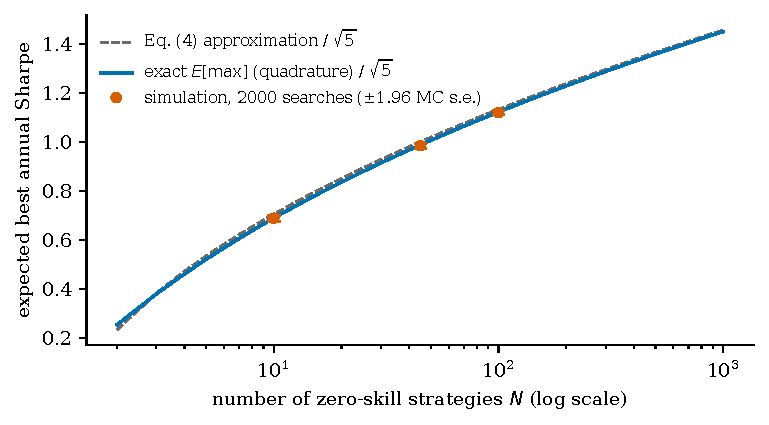
\includegraphics[width=0.78\textwidth]{figures/fig1_best_of_n.pdf}
\caption{Expected best annualized Sharpe ratio among $N$ zero-skill IID Normal strategies over five years of 250 daily returns. Curves: the approximation Eq.~\eqref{eq:emax} and exact quadrature, both divided by $\sqrt5$. Points: D1 simulation, 2000 searches per $N$, with $\pm1.96$ Monte Carlo standard errors. The approximation exceeds the exact value by 0.016 at $N=10$; the simulation agrees with the exact value. Source: \texttt{results/best\_of\_n.txt}; curves evaluated analytically.}\label{fig:bestofn}
\end{figure}

\section{Empirical results}\label{sec:results}

\subsection{IID baseline and selection: PSR versus DSR}\label{sec:res:dsr}

\emph{What was tested.} Whether PSR(0) and DSR flag the winner of a zero-skill search (D2) and a fixed strategy (D3, IID row). \emph{Why.} PSR ignores the search; DSR is designed to correct for it.

On a fixed IID Normal strategy, PSR(0)$>0.95$ occurs in 4.95\% [4.04, 5.99] of 2000 datasets: the asymptotic 5\% reading holds at $T=1248$. Applied to the best of 100 zero-skill strategies, PSR(0)$>0.95$ occurs in 99.15\% [98.64, 99.50] of searches. DSR$>0.95$ occurs in 0.05\% [0.00, 0.28] (1 of 2000), and the mean DSR of the winner is 0.488.

\emph{Interpretation.} This is a property of the 2014 construction, not a calibration failure. The winner's Sharpe is centred near $\SR_0$, so DSR is centred near one half. Its spread is that of a single strategy's estimation error, $(T-1)^{-1/2}$, whereas the maximum of $N$ IID Normals has a smaller spread than any one of them. A one-sided hurdle at 0.95 in units of the wider spread is therefore rarely crossed. A closed-form approximation treating $V$ as known gives 0.15\%, consistent with the simulation. DSR(0.95) is thus a conservative screen under this null, not a 5\% test. Neither \citet{bailey2014dsr} nor \citet{lopezdeprado2026porcu} claims a 5\% size for this rule; the latter describe the location benchmark as one of several constructions with different objectives.

\subsection{Serial dependence, GARCH, heavy tails and correlation}\label{sec:res:calib}

\emph{What was tested.} H1, H3 and H4 in D3: each scenario departs from IID Normality in one named respect, with zero true edge throughout. Table~\ref{tab:calibration} reports all cells and Figure~\ref{fig:calibration} plots the rejection rates.

\begin{table}[t]
\centering\small
\begin{threeparttable}
\footnotesize\setlength{\tabcolsep}{4pt}
\caption{Zero-edge synthetic calibration (D3). Rates in \% with exact 95\% intervals, 2000 datasets per cell. Mean PBO $\pm$ one Monte Carlo s.e., 200 datasets. $N=100$, $T=1248$, $S=16$.}\label{tab:calibration}
\begin{tabular}{@{}lccccc@{}}
\toprule
Scenario & PSR(0)$>0.95$ & PSR, Newey--West & DSR, $N=100$ & DSR, $\hat N$ & Mean PBO \\
\midrule
IID Normal & 4.95 [4.04, 5.99] & 5.10 & 0.00 [0.00, 0.18] & & $0.520\pm0.010$ \\
AR(1) $\phi=0.1$ & 6.35 [5.32, 7.51] & 5.30 & 0.10 [0.01, 0.36] & & $0.495\pm0.010$ \\
AR(1) $\phi=0.3$ & 11.85 [10.47, 13.35] & 7.10 [6.01, 8.31] & 0.70 [0.38, 1.17] & & $0.482\pm0.011$ \\
GARCH (0.05, 0.90) & 4.70 [3.81, 5.72] & 4.60 & 0.15 [0.03, 0.44] & & $0.481\pm0.011$ \\
GARCH (0.10, 0.85) & 5.45 [4.50, 6.54] & 5.80 & 0.10 [0.01, 0.36] & & $0.501\pm0.011$ \\
Student-$t$, $\nu=8$ & 4.35 [3.50, 5.34] & 4.65 & 0.15 [0.03, 0.44] & & $0.511\pm0.011$ \\
Student-$t$, $\nu=5$ & 4.85 [3.95, 5.88] & 5.20 & 0.05 [0.00, 0.28] & & $0.504\pm0.011$ \\
Equicorr.\ $\rho=0.3$ & 5.35 [4.40, 6.43] & 5.55 & 0.70 [0.38, 1.17] & 1.05 [0.65, 1.60] & $0.512\pm0.011$ \\
Equicorr.\ $\rho=0.7$ & 4.95 [4.04, 5.99] & 5.20 & 2.60 [1.95, 3.40] & 5.05 [4.13, 6.10] & $0.504\pm0.011$ \\
\bottomrule
\end{tabular}
\begin{tablenotes}\footnotesize
\item PSR is computed on a fixed strategy, DSR on the full-sample winner. $\hat N$ is Eq.~\eqref{eq:impliedn}; its mean is 70.3 at $\rho=0.3$ and 30.7 at $\rho=0.7$. Newey--West uses 7 Bartlett lags. Exact binomial tests of the PSR column against 5\%, Holm over nine scenarios: $\phi=0.3$ detected ($p<10^{-4}$); $\phi=0.1$ suggestive (exact $p=0.0075$, Holm $p=0.060$); all others not different from 5\% (Holm $p=1$). PBO$\le0.05$ accepted a zero-edge set in at most 1 of 200 datasets in any scenario. Source: \texttt{results/calibration.txt}, \texttt{results/manuscript\_numbers.txt}.
\end{tablenotes}
\end{threeparttable}
\end{table}

\begin{figure}[t]
\centering
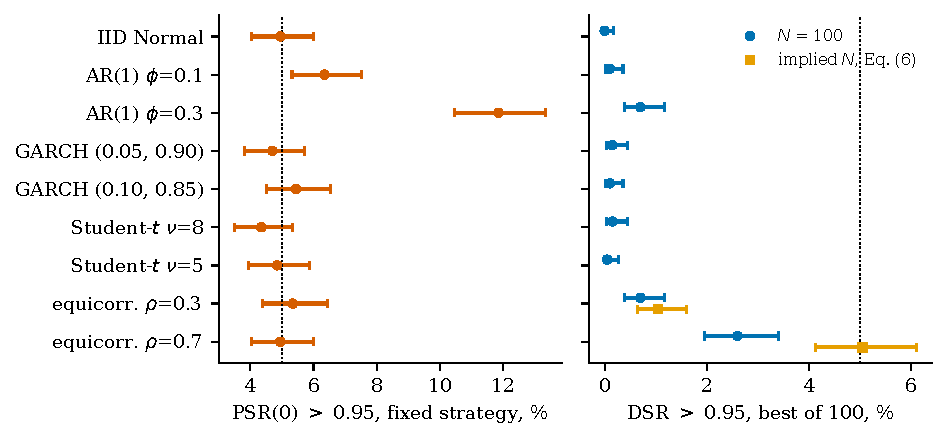
\includegraphics[width=0.92\textwidth]{figures/fig3_calibration.pdf}
\caption{Rejection rates under zero true edge across the D3 scenarios, with exact 95\% intervals (2000 datasets per point). Left: uncorrected PSR(0)$>0.95$ on a fixed strategy. Right: DSR$>0.95$ on the best of 100, with $N=100$ and, in correlated designs, with the interpolated $\hat N$. The dotted line is 5\%. Only AR(1) moves PSR; only cross-strategy correlation moves DSR materially. Source: \texttt{results/calibration.txt}.}\label{fig:calibration}
\end{figure}

\paragraph{PSR and serial dependence.} H1 is rejected for AR(1) $\phi=0.3$ and is suggestive for $\phi=0.1$; it is not rejected for any other scenario. The observed rates agree with Proposition~\ref{prop:rate}: 6.35\% against 6.84\% and 11.85\% against 11.37\%, both inside the simulated intervals (Figure~\ref{fig:psrar1}). H2 is therefore supported in the synthetic design. GARCH returns are serially uncorrelated, so $F=1$ and, at $\SR=0$, the kurtosis term in Eq.~\eqref{eq:mertens} vanishes; the GARCH and Student-$t$ cells being near 5\% is what theory predicts at $\SR^\ast=0$ and says nothing about PSR at $\SR^\ast>0$, where kurtosis and volatility clustering do enter \citep{lopezdeprado2026garch}.

\paragraph{Newey--West correction.} With 7 Bartlett lags the $\phi=0.3$ rate falls to 7.10\% [6.01, 8.31], not to 5\%. Truncation bias alone, an expected Bartlett factor of 1.704 against the true 1.857, predicts 5.76\%, below the simulated interval; the remaining excess is consistent with the added sampling variability of $\hat F_\ell$, which the Normal approximation ignores. Longer bandwidths, prewhitening and fixed-$b$ critical values \citep{kiefer2005} were not tried. In every other scenario the corrected rate is within its interval of 5\%.

\begin{figure}[t]
\centering
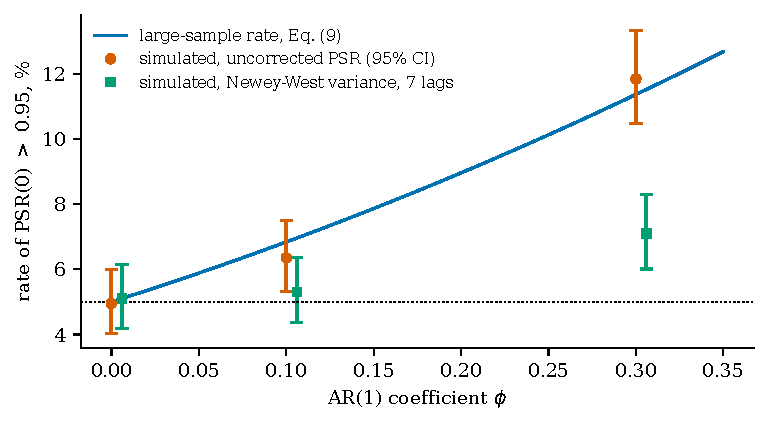
\includegraphics[width=0.78\textwidth]{figures/fig2_psr_ar1.pdf}
\caption{Uncorrected PSR(0)$>0.95$ rejection rate for a zero-Sharpe Gaussian AR(1), $T=1248$. Line: large-sample rate from Eq.~\eqref{eq:ar1rate}, an asymptotic approximation evaluated analytically. Circles: D3 simulation (2000 datasets each, exact 95\% intervals). Squares: the same datasets with a Newey--West variance (7 lags), offset horizontally for legibility. Dotted line: 5\%. Source: \texttt{results/calibration.txt}, \texttt{results/psr\_ar1\_curve.txt}.}\label{fig:psrar1}
\end{figure}

\paragraph{DSR and correlated strategies.} H3 is rejected in the opposite direction from the usual concern: in seven of nine scenarios DSR rejects in at most 0.70\% of searches. The exception is cross-strategy correlation. Writing returns as $r_{it}=\sqrt{\rho}\,f_t+\sqrt{1-\rho}\,e_{it}$, the trial Sharpes share the common component, so the cross-sectional variance $V$ measures only the idiosyncratic dispersion, of order $(1-\rho)/T$. $\SR_0=\sqrt V\,\E[\max_N]$ then shrinks, while the selected Sharpe still carries the common shock, whose variance is of order $\rho/T$. DSR acceptance rises to 2.60\% at $\rho=0.7$ with $N=100$, and to 5.05\% with $\hat N=30.7$. The 5.05\% figure is where this design happens to cross 5\%, not evidence that Eq.~\eqref{eq:impliedn} recovers a true number of independent trials: for this one-factor design the expected maximum is exactly $\sqrt{1-\rho}$ times the IID value, 1.373 at $N=100,\rho=0.7$, whereas the implemented approximation with $\hat N=30.7$ and $V=0.3$ gives 1.141 (standardized units). Recovering $\hat N=30.715\pm0.019$ checks the estimate of Eq.~\eqref{eq:impliedn}, not the correction it feeds.

\paragraph{PBO.} H4 holds in every scenario: mean PBO is within about two standard errors of 1/2, and PBO$\le0.05$ accepted a zero-edge set at most once in 200 datasets. Because the strategies are exchangeable and no scenario creates dependence between IS and OOS halves, a mean of one half is guaranteed here; these nulls do not stress the mechanism by which PBO detects overfitting. Paired time-shuffle controls under GARCH give $-0.002\pm0.004$ and $+0.009\pm0.004$.

\paragraph{PBO with one true edge (D5, exploratory).} Mean PBO falls from 0.516 at $\SR_a=0$ to 0.433, 0.189 and 0.026 at $\SR_a=1,2,3$ under IID noise. Under AR(1) $\phi=0.3$ noise it is higher at $\SR_a=2$ ($0.391\pm0.043$ versus $0.189\pm0.037$) and $\SR_a=3$ ($0.098\pm0.019$ versus $0.026\pm0.007$); no change is detected under GARCH. The edge was held fixed as a daily mean-to-SD ratio. Under AR(1) the same daily ratio is a weaker signal at horizons comparable to the CSCV halves: the label $\SR_a=2$ corresponds to a 250-day summed-return Sharpe of 1.47. That alone can account for much of the shift. Only mean PBO was measured, not the probability of passing PBO$\le0.05$ or of selecting the planted strategy, and 20 skewed values per cell make Normal-theory comparisons rough. We therefore draw no conclusion about PBO's decision power under dependence.

\subsection{Historical market data: block bootstrap of industry returns}\label{sec:res:real}

\emph{What was tested.} H1 and H2 on real dependence (D4). \emph{Why.} Synthetic AR(1) is a stylized departure; the question is whether the dependence in actual daily returns is large enough to matter and whether Eq.~\eqref{eq:blockF} predicts it. Table~\ref{tab:real} reports every run, and Figure~\ref{fig:real} plots them.

\begin{table}[t]
\centering\small
\begin{threeparttable}
\caption{PSR(0)$>0.95$ on block-bootstrapped industry returns with zero true edge (D4). $T=1248$, 2000 datasets per row, PSR on a uniformly drawn industry.}\label{tab:real}
\begin{tabular}{@{}lccccl@{}}
\toprule
Run & Rate, \% [95\% CI] & Approx., \% & Exact $p$ & Holm $p$ & Verdict \\
\midrule
Full window, $L=1$ & 5.35 [4.40, 6.43] & 4.99 & 0.47 & 0.94 & none \\
Full window, $L=5$ & 5.15 [4.22, 6.21] & 5.42 & 0.76 & 0.94 & none \\
Full window, $L=20$ & 6.25 [5.23, 7.40] & 5.50 & 0.014 & 0.055 & suggestive \\
Full window, $L=60$ & 6.25 [5.23, 7.40] & 5.38 & 0.014 & 0.055 & suggestive \\
Replicate, $L=20$ & 5.90 [4.91, 7.02] & 5.50 & 0.072 & 0.090 & none \\
Replicate, $L=60$ & 6.00 [5.00, 7.13] & 5.38 & 0.045 & 0.090 & suggestive \\
\midrule
1971--1998, centred, $L=20$ & 8.35 [7.17, 9.65] & 8.37 & $<10^{-4}$ & $<10^{-4}$ & detected (above) \\
1999--2026, centred, $L=20$ & 3.85 [3.05, 4.79] & 3.94 & 0.018 & 0.018 & detected (below) \\
\bottomrule
\end{tabular}
\begin{tablenotes}\footnotesize
\item Approximation: $\pi(F^{\mathrm{boot}})$ from Eq.~\eqref{eq:blockF} with each industry's circular autocorrelations, averaged over industries (our derivation). Holm families: first run (4 rows), replicate (2), sub-periods (2). The full-window approximations were saved before a partial-block correction that changes them by at most 0.01 points. Sub-period counts are 167/2000 and 77/2000. Sources: \texttt{results/french\_bootstrap.txt}, \texttt{french\_followups.txt}, \texttt{g6\_corrected.txt}, \texttt{manuscript\_numbers.txt}.
\end{tablenotes}
\end{threeparttable}
\end{table}

\begin{figure}[t]
\centering
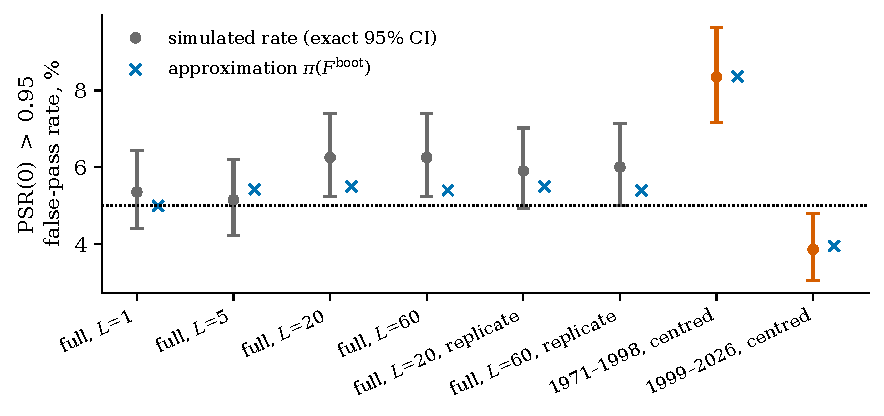
\includegraphics[width=0.85\textwidth]{figures/fig4_real_data.pdf}
\caption{PSR(0)$>0.95$ on block-bootstrapped daily industry returns with zero true edge (D4), with exact 95\% intervals (2000 datasets per point). Crosses: autocorrelation approximation $\pi(F^{\mathrm{boot}})$, Eqs.~\eqref{eq:ar1rate}--\eqref{eq:blockF}. The two right-hand points resample each period after centring each industry within that period. Intervals are Monte Carlo error conditional on the observed history. Source: \texttt{results/french\_bootstrap.txt}, \texttt{french\_followups.txt}, \texttt{g6\_corrected.txt}.}\label{fig:real}
\end{figure}

\emph{Observation.} On the full 1971--2026 history, the excess is at most suggestive (6.25\% at $L=20$ and $60$; 5.90\% and 6.00\% in the replicate). Splitting the history shows why. Mean daily lag-1 autocorrelation across industries was $+0.157$ in 1971--1998 (all 49 industries significantly positive) and $-0.026$ in 1999--2026. Resampling the early period with each industry centred, PSR rejects 8.35\% [7.17, 9.65]; resampling the late period it rejects 3.85\% [3.05, 4.79]. Both intervals exclude 5\%, in opposite directions. Descriptively, the full-window rate is close to the simple average of the two (6.1\%); this is an observation, not a decomposition of the bootstrap rates, but it suggests the full-window figure describes neither period. In both periods the autocorrelation approximation is within 0.1 percentage points of the simulation (8.37\% and 3.94\%) and inside its interval.

\emph{Uncertainty and status.} These intervals are Monte Carlo error given one history and one bootstrap design; they are not confidence intervals for a population rejection rate across market histories. No decision rule for the direction of the sub-period effects was fixed before the run, and the recorded prediction equals the approximation and was proposed after an earlier, uncorrected run was seen. The agreement is therefore a model check of Eq.~\eqref{eq:blockF}, not an independent confirmation. The earlier run, which did not centre each period, is withdrawn (Appendix~\ref{app:corrections}).

\emph{Corrections.} Applying a Newey--West variance to the replicate datasets gives 5.60\% and 5.70\% at $L=20$ and 60, and using AR(5) residuals gives 5.30\% and 5.35\%; all contain 5\%. These are robustness checks, not isolated interventions: residual filtering also changes marginal moments and cross-industry relationships. Weekly five-day sums give 4.35\% [3.50, 5.34] but change horizon, sample span and moments at the same time.

\emph{DSR and PBO on industries.} DSR acceptance stays below 5\% throughout: 3.05--3.55\% with $\hat N$ (mean 23.0--23.3 for 49 industries) and 1.25--1.90\% with $N=49$. Mean PBO is 0.505--0.520 against the reference $25/49=0.510$, with Monte Carlo s.e.\ 0.012--0.014. A time-shuffle control gave $+0.017\pm0.005$ at $L=60$ in the first run; that effect did not replicate in 400 further datasets ($+0.001\pm0.004$ with fixed block positions, $-0.001\pm0.004$ with random positions).

\emph{Alternative explanation.} The pre-1999 autocorrelation is plausibly in part a nonsynchronous-trading effect in portfolio returns \citep{lo1990}, and decimalization and higher trading volume after 1999 are candidate reasons for its disappearance. It is real dependence in the series to which PSR is applied, whatever its source, but not necessarily exploitable predictability. We did not test the mechanism.

\subsection{Strategy-search case study}\label{sec:res:case}

\emph{What was tested.} H5: whether the best of 93 moving-average settings has a higher Sharpe ratio than buy-and-hold after accounting for dependence and for the search (D6). \emph{Why.} DSR and PBO are routinely reported for such searches; neither compares the winner with the market.

Recorded predictions, made before the run, were: PBO between 0.05 and 0.5; DSR above 0.95; PBO roughly unchanged across costs; and an in-sample Sharpe above the market's. Table~\ref{tab:case} reports the results. The first, second and fourth predictions were correct; the third was not judged because no tolerance was set in advance.

\begin{table}[t]
\centering\small
\begin{threeparttable}
\caption{Strategy search on the US market factor (D6). 93 settings, 18 July 1972 to 30 September 2026, $T=13{,}664$. Sharpe ratios annualized by $\sqrt{250}$.}\label{tab:case}
\begin{tabular}{@{}lccc@{}}
\toprule
& 0 bps & 5 bps (main) & 10 bps \\
\midrule
Selected setting (fast/slow) & 15/225 & 15/225 & 15/225 \\
Its Sharpe ratio & 0.593 & 0.588 & 0.582 \\
Buy-and-hold Sharpe ratio & 0.458 & 0.458 & 0.458 \\
Settings above buy-and-hold & 55 of 93 & 50 of 93 & 45 of 93 \\
PSR(0) of the selected setting & 1.0000 & 1.0000 & 1.0000 \\
DSR, $N=93$ & 0.9985 & 0.9980 & 0.9969 \\
DSR, $\hat N=17.2$ & 0.9995 & 0.9994 & 0.9991 \\
PBO ($S=16$) & 0.240 & 0.208 & 0.193 \\
\midrule
\multicolumn{4}{@{}l}{\emph{Paired HAC test against buy-and-hold, 5 bps, selected setting}} \\
Bartlett lags & 0 & 11 (primary) & 44 \\
Difference (s.e.) & 0.130 (0.104) & 0.130 (0.099) & 0.130 (0.101) \\
95\% CI & [$-0.073$, 0.333] & [$-0.064$, 0.323] & [$-0.069$, 0.329] \\
One-sided $p$, unadjusted & 0.105 & 0.094 & 0.100 \\
Bonferroni-adjusted $p$ & 1.000 & 1.000 & 1.000 \\
Settings passing Bonferroni & 0 of 93 & 0 of 93 & 0 of 93 \\
\bottomrule
\end{tabular}
\begin{tablenotes}\footnotesize
\item Sources: \texttt{results/ma\_crossover.txt}, \texttt{market\_comparison.txt}, \texttt{manuscript\_numbers.txt}. The unadjusted $p$ of the selected setting is itself selection-biased; it is the smallest of the 93.
\end{tablenotes}
\end{threeparttable}
\end{table}

\paragraph{Search-adjusted statistics.} The winner's DSR is 0.998 with $N=93$ and 0.999 with $\hat N=17.2$: its Sharpe is far above $\SR_0$, the expected best of 93 zero-skill trials. This is unsurprising and mostly mechanical. Over 54 years of daily data the standard error of a daily Sharpe is about $(13{,}664)^{-1/2}\approx0.0086$, and the 93 settings are closely related, so $V$ and $\SR_0$ are small; almost any rule that is long the equity premium most of the time clears the zero-skill benchmark. Holding $V$ fixed, DSR falls below 0.95 only at $N\approx7.4\times10^5$ trials (Figure~\ref{fig:dsrn}). PBO is 0.208: in 20.8\% of the 12,870 CSCV splits, the IS winner ranked at or below the OOS median among the 93 settings. It fails the customary 0.05 cut-off, but there is no reference distribution for PBO in a correlated rule family, and in D5 a planted true edge of $\SR_a=2$ also produced mean PBO near 0.19; the cut-off rejects real edges too.

\paragraph{Benchmark-relative test.} Figure~\ref{fig:grid} shows the full surface of Sharpe differences, and Figure~\ref{fig:z} the 93 $z$-statistics. 43 of 93 differences are negative. The selected setting's advantage is $+0.130$ (s.e.\ 0.099, 95\% CI $[-0.064, 0.323]$, one-sided $p=0.094$). No setting passes the Bonferroni threshold $z>3.270$; the largest $z$ is 1.31. The decision is the same at 0 and 44 lags. H5 is not rejected.

\emph{Power.} Under a Normal-shift approximation that holds the estimated s.e.\ of 0.099 fixed, a single one-sided 5\% test has 80\% power only against a true difference of 0.246, and the Bonferroni test only against 0.406; the implied power against a true difference of 0.130 is 0.37 unadjusted and 0.025 after Bonferroni. These are illustrative calculations for the selected setting's test, not measured power of the full search-and-selection procedure. Failure to reject therefore establishes insufficient evidence of superiority, not the absence of timing skill.

\begin{figure}[t]
\centering
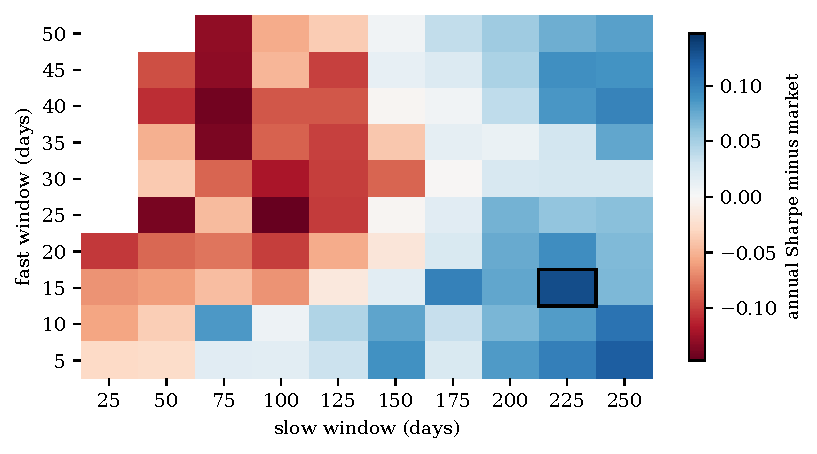
\includegraphics[width=0.8\textwidth]{figures/fig5_grid.pdf}
\caption{Annualized Sharpe ratio of each moving-average setting minus that of buy-and-hold, 5 bps, 1972--2026 (D6). The boxed cell is the in-sample winner, 15/225. Blank cells have fast $\ge$ slow. Positive differences cluster at long slow windows, which spend most days long the market. Source: \texttt{results/market\_comparison.txt}.}\label{fig:grid}
\end{figure}

\begin{figure}[t]
\centering
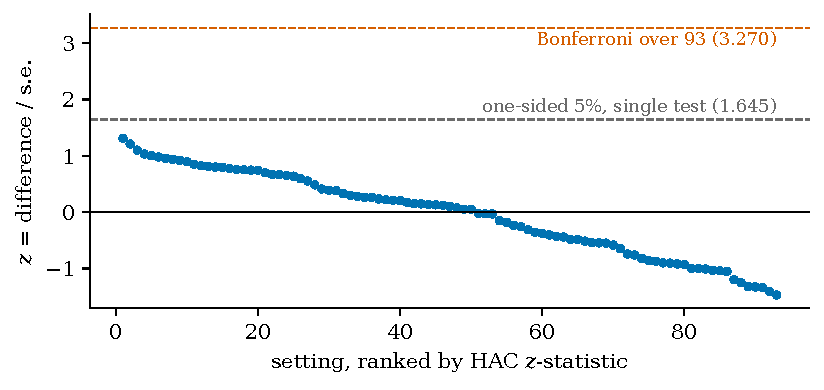
\includegraphics[width=0.8\textwidth]{figures/fig6_z.pdf}
\caption{Paired HAC $z$-statistics (11 Bartlett lags) for all 93 settings against buy-and-hold, ranked. The largest is 1.31 (setting 15/225); the Bonferroni threshold at family level 5\% is 3.270. Source: \texttt{results/market\_comparison.txt}.}\label{fig:z}
\end{figure}

\paragraph{Data-snooping test.} Bonferroni is conservative when the 93 statistics are strongly correlated, as here. Hansen's SPA test, which accounts for that correlation through a joint stationary bootstrap, gives $T^{\mathrm{SPA}}=1.265$ and $p=0.504$. The conclusion does not depend on the multiplicity correction.

\section{Robustness and sensitivity}\label{sec:robust}

All checks in this section are exploratory (Table~\ref{tab:classification}). They use 5 bps and 11 lags unless stated; Table~\ref{tab:robust} reports them.

\begin{table}[t]
\centering\small
\begin{threeparttable}
\caption{Case-study robustness (D7). Annualized Sharpe ratios and differences; paired tests with 11 Bartlett lags.}\label{tab:robust}
\begin{tabularx}{\textwidth}{@{}>{\raggedright\arraybackslash}p{4.3cm}>{\raggedright\arraybackslash}X@{}}
\toprule
Check & Result \\
\midrule
Baseline (signal acts next day) & 15/225: Sharpe 0.588 vs 0.458; PBO 0.208; DSR 0.9980; difference $+0.130$, $p=0.094$ \\
One extra day of execution lag & 15/225 still selected: Sharpe 0.578; PBO 0.216; DSR 0.9959; difference $+0.120$ (s.e.\ 0.099), $p=0.113$; 48 of 93 above market \\
Turnover of 15/225 & 72 position changes in 54.7 years, 1.32 per year; long on 76\% of days \\
Break-even cost & 121 bps per change before its Sharpe equals the market's \\
1972--1998 (6,686 days) & Sharpe 0.568 vs 0.500; difference $+0.068$ (s.e.\ 0.134), $p=0.305$ \\
1999--2026 (6,978 days) & Sharpe 0.606 vs 0.439; difference $+0.167$ (s.e.\ 0.140), $p=0.117$ \\
DSR break-even trial count & DSR $<0.95$ only for $N\gtrsim7.4\times10^5$, $V$ fixed \\
Hansen SPA, 93 settings & $T^{\mathrm{SPA}}=1.265$, $p=0.504$ \\
Walk-forward, 1982--2026 & Re-selected each January on all prior data: OOS Sharpe 0.466 vs market 0.536; difference $-0.070$ (s.e.\ 0.107), one-sided $p=0.74$; 10 distinct settings chosen \\
\bottomrule
\end{tabularx}
\begin{tablenotes}\footnotesize
\item Sources: \texttt{results/case\_study\_checks.txt}, \texttt{results/performance\_checks.txt}. The walk-forward sample (11,276 days) differs from the full sample, so its market Sharpe differs from 0.458.
\end{tablenotes}
\end{threeparttable}
\end{table}

\paragraph{Execution lag and costs.} The selected rule trades about once a year. One additional day of delay lowers its Sharpe by 0.010 and leaves it the winner; costs between 0 and 10 bps move its Sharpe by 0.011. Trading frictions of plausible size are therefore not what separates the rule from the market. The break-even cost of 121 bps per change is far above realistic index-trading costs. The cost model is a flat charge per unit turnover and ignores market impact, financing and taxes.

\paragraph{Lag specification.} The HAC standard error moves from 0.104 (0 lags) to 0.099 (11) to 0.101 (44). The market factor's daily lag-1 autocorrelation over the sample is $-0.001$. The decision does not depend on bandwidth.

\paragraph{Sub-periods.} The in-sample advantage is larger after 1999 ($+0.167$) than before ($+0.068$), so the pre-1999 stale-price autocorrelation documented in Section~\ref{sec:res:real} does not explain it. Neither sub-period difference is significant, and each has a standard error of about 0.14.

\paragraph{Walk-forward selection.} When the setting is re-selected each January using only past data, the resulting strategy earns an out-of-sample Sharpe of 0.466 over 1982--2026 against the market's 0.536 over the same days, with costs charged on the actual held positions, including at rule switches. The full-sample advantage of the in-sample winner (+0.130) becomes a shortfall ($-0.070$, s.e.\ 0.107). The walk-forward design was not recorded before it ran, and one realized path is weak evidence. It is consistent with the PBO of 0.208 indicating unstable rankings and with the failure of the benchmark tests, and it is the only check here that does not reuse the selection sample.

\paragraph{Multiple-testing sensitivity.} The selected setting fails at the unadjusted one-sided 5\% level, so no correction is needed to reach the decision. Bonferroni and the joint SPA test agree. A Romano--Wolf stepwise procedure, which would identify individual outperforming rules, was not run, and its outcome is not reported.

\begin{figure}[t]
\centering
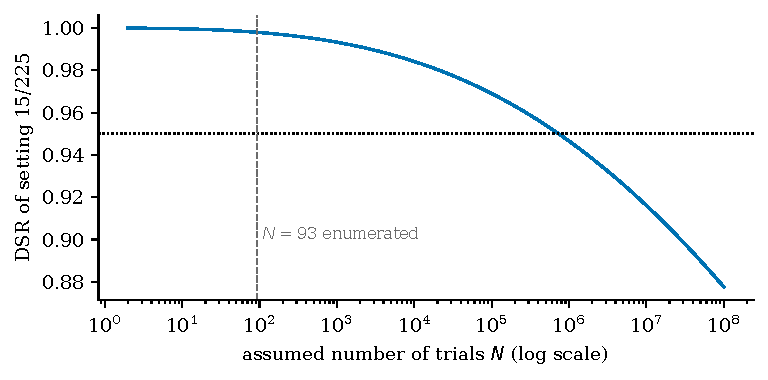
\includegraphics[width=0.78\textwidth]{figures/fig7_dsr_vs_n.pdf}
\caption{DSR of setting 15/225 as a function of the assumed number of trials $N$, holding the observed $V$, skewness, kurtosis and $T=13{,}664$ fixed. The dotted line is 0.95; the dashed line marks the 93 settings actually tried. Evaluated from Eqs.~\eqref{eq:psr}--\eqref{eq:dsr}; source: \texttt{results/fig7\_dsr\_vs\_n.txt}.}\label{fig:dsrn}
\end{figure}

\section{Discussion}\label{sec:discussion}

\paragraph{What the evidence establishes.} Within the designs studied, the three statistics behave as their constructions imply, and none answers the question a capital allocator usually asks. Uncorrected PSR is a valid asymptotic 5\% test at $\SR^\ast=0$ when the returns it uses are serially uncorrelated; with dependence its size is $\pi(F)$, which can be above or below 5\%. The 2014 DSR is a conservative screen against a zero-skill benchmark whose acceptance rate depends on cross-strategy correlation and on the trial-count convention. PBO measures rank persistence inside the candidate set and reproduces its exchangeable reference under every zero-edge null tried. The case study shows the practical consequence: DSR 0.998, a CSCV result that fails the 0.05 rule, and no evidence of beating the market are mutually consistent, because they test different hypotheses.

\begin{table}[t]
\centering\small
\caption{Which statistic answers which question.}\label{tab:decision}
\begin{tabularx}{\textwidth}{@{}>{\raggedright\arraybackslash}p{3.4cm}>{\raggedright\arraybackslash}p{2.6cm}>{\raggedright\arraybackslash}X>{\raggedright\arraybackslash}X@{}}
\toprule
Decision & Statistic & A pass does not imply & Evidence still needed \\
\midrule
Is one pre-specified Sharpe above a hurdle? & PSR($\SR^\ast$) & Robustness to serial dependence (Secs.~\ref{sec:res:calib}, \ref{sec:res:real}) & HAC variance or lower frequency, checked for the period \\
Is a search winner better than the best of $N$ noise trials? & DSR (2014) & A 5\% error rate; skill relative to a benchmark & A defensible $N$; a benchmark-relative test \\
Do the search's rankings persist out of sample? & PBO & A probability of future loss & A reference distribution for the rule family \\
Should capital move from the benchmark to the strategy? & None of the above & & Search-aware benchmark test (Reality Check, SPA, StepM) with power; walk-forward evidence; costs and capacity \\
\bottomrule
\end{tabularx}
\end{table}

\paragraph{Why the methods behave differently.} PSR's only route to miscalibration at $\SR^\ast=0$ is the variance of the sample mean, so only autocorrelation matters; heavy tails and volatility clustering enter through terms multiplied by $\SR$ and vanish at the null tested. DSR's benchmark is a location shift of a single-strategy distribution, so its size depends on how the spread of the maximum compares with the spread of one estimate, and on how much common variation $V$ omits. CSCV compares ranks within a set, so any common component cancels and only relative persistence matters.

\paragraph{Financial interpretation.} The moving-average rule mainly reduces exposure in prolonged declines: it is long 76\% of days and has lower volatility than the market (12.1\% against 16.9\% a year, Appendix~\ref{app:tables}). A higher Sharpe for a lower-volatility, long-biased variant of the market is a familiar pattern and does not by itself demonstrate predictability. Its in-sample advantage is not statistically distinguishable from zero and reverses under walk-forward selection. Our evidence is weaker than that of \citet{sullivan1999}, whose best Dow Jones rule did survive a data-snooping adjustment in sample before failing out of sample; here the in-sample advantage is already insignificant, and the walk-forward result points in the same direction as their out-of-sample finding.

\paragraph{Statistical interpretation.} Two lessons generalize. First, fixed correction factors are inadequate when dependence changes over time; the same industry data imply rejection rates of 8.4\% and 3.9\% depending on the period. Second, a hurdle on a selection-adjusted zero-skill statistic is not a hypothesis test against an investable alternative. A benchmark-relative question needs a benchmark-relative test, and that test should report its power.

\paragraph{Comparison with prior literature.} The AR(1) result confirms \citet{lo2002} and \citet[Remark~3.1]{ledoit2008}. The walk-forward shortfall is consistent with the out-of-sample failure reported by \citet{sullivan1999}, although our in-sample evidence was never significant. The DSR operating characteristics are, to our knowledge, not tabulated in the 2014 paper; \citet{lopezdeprado2026porcu} derive general calibration results for DSR variants, and their full text, which we have not read, may contain equivalent or more general findings. We therefore do not claim priority for them.

\paragraph{What the results do not establish.} They do not establish the size of PSR at $\SR^\ast>0$, the behaviour of MinTRL under dependence, the decision power of PBO, the performance of later DSR variants, the absence of timing skill in moving-average rules, or anything about future returns.

\section{Limitations}\label{sec:limits}

\begin{itemize}
\item \textbf{Dataset representativeness.} Real-data results use one data vendor's US industry and market portfolios over 1971--2026. Other markets, frequencies, or individual securities may have different dependence.
\item \textbf{Regime changes.} The sub-period analysis shows that the dependence structure is not stable. Any bootstrap with a fixed block length assumes stationarity within the resampled window; the circular block bootstrap with fixed blocks is not itself stationary across block positions and removes dependence beyond $L$. Block lengths were fixed by design, not chosen by a data-driven rule such as \citet{politis2004}.
\item \textbf{Data construction.} The French portfolios are built from CRSP, which includes delisted firms, so survivorship is not a concern at the portfolio level. The research factors are computed with today's vintage of CRSP data and the library's current methodology; they are not point-in-time series that a trader could have observed, and revisions between releases change history.
\item \textbf{Model assumptions.} Synthetic levels are our choices. Only $\SR^\ast=0$ was tested for PSR. HAC inference requires stationarity, mixing and finite moments that the market history may violate (raw kurtosis 17.7).
\item \textbf{Exploratory and post hoc analysis.} The evidence rule was finalized after results were known; the sub-period prediction was not blind; the D7 checks have no recorded predictions; the walk-forward design was not recorded before running. No analysis was registered with a third party.
\item \textbf{No prospective validation.} All tests use historical data. The walk-forward check is pseudo-out-of-sample on one path and uses a rule family chosen with knowledge of the literature.
\item \textbf{Monte Carlo resolution.} With 2000 datasets, effects smaller than about one percentage point in a rejection rate are not resolved; PBO cells use 200 datasets and D5 only 20.
\item \textbf{Strategy realism.} Same-close fills on a research portfolio, flat costs, no capacity, financing or tax effects. The case study is a statistical illustration, not an implementable strategy.
\item \textbf{Literature access.} Three 2026 papers in the same lineage were examined only through abstracts and metadata. Two older working papers (Mertens 2002; Memmel 2003) were not examined directly.
\item \textbf{Reproducibility.} Both exact data archives have timestamped, hash-verified recovery URLs (Section~\ref{sec:repro}); long-term archival availability and provider data terms remain external dependencies.
\item \textbf{Novelty.} The serial-dependence mechanism, the SPA test and the technical-rule conclusion are established. The contribution is replication, quantified operating characteristics in specific designs, and their juxtaposition.
\end{itemize}

\section{Data, code and reproducibility}\label{sec:repro}

Saved outputs were regenerated from the corrected code in an isolated environment and compared with the archived outputs (Appendix~\ref{app:repro}). The historical \texttt{french\_followups.txt} is intentionally retained: three displayed approximations differ from the current partial-block formula, while all simulated counts agree. The corrected walk-forward output and its original predecessor are stored separately. The current suite contains 285 passing tests. Both input ZIPs have independently retrieved, SHA-256-verified Internet Archive captures: industry capture \texttt{20261113053423} and factor capture \texttt{20261030074337}. Data are not redistributed with the code or licensed under its MIT licence. Archive availability does not grant data redistribution rights or guarantee perpetual access. Detailed clean-environment verification and source-version information accompany this release.

\section{Conclusion}\label{sec:conclusion}

We asked how reliable standard backtest-validation statistics are under realistic departures from their assumptions, and whether a historically superior rule survives selection-aware testing. Replicated results: the selected numerical examples of Table~\ref{tab:replication} are reproduced, and uncorrected PSR over-rejects under AR(1) dependence at the rate long-run-variance theory predicts, as already known. Empirical extensions: on daily US industry returns PSR's error depends on the period's dependence and runs in both directions, and a simple autocorrelation approximation predicts it; the 2014 DSR is far from a 5\% test under IID zero-skill searches and becomes less conservative as strategies become correlated; PBO reproduces its exchangeable reference under every zero-edge null tried. In a search over 93 moving-average rules on the US market factor, the selected rule has DSR 0.998 but no evidence of outperforming buy-and-hold, under a paired HAC test, Bonferroni and Hansen's SPA, and it underperforms the market under walk-forward re-selection. These statistics answer different questions, and a high value on one of them should not be read as evidence of an investable edge. Nothing here bears on future performance.

\section*{Statements}
\textbf{Data availability.} Kenneth R.\ French Data Library, daily 49 Industry Portfolios and Fama--French research factors, 202609 CRSP release, downloaded 12 November 2026; SHA-256 in Appendix~\ref{app:repro}. \textbf{Code availability.} The repository accompanying this paper (MIT licence); the exact commit is to be recorded with any public release. \textbf{Funding, conflicts of interest.} None declared. \textbf{Ethics.} Not applicable: public aggregate data, no human subjects.

\bibliographystyle{plainnat}
\bibliography{references}

\appendix

\section{Derivations}\label{app:derivations}

\paragraph{Proposition~\ref{prop:rate}.} Write $\hSR=\bar r/\hat\sigma$. Under $\mu=0$, $\sqrt T\bar r/\sigma\to\mathcal N(0,F)$ by a CLT for stationary weakly dependent sequences, and $\hat\sigma\to\sigma$ in probability, so $\sqrt T\hSR\to\mathcal N(0,F)$ by Slutsky's theorem. Since $\hSR\to0$, the PSR denominator in Eq.~\eqref{eq:psr} tends to 1 and $\sqrt{(T-1)/T}\to1$; hence the PSR $z$-statistic converges to $\mathcal N(0,F)$ and $\Pr(z>z_{1-\alpha})\to1-\Phi(z_{1-\alpha}/\sqrt F)$. For AR(1), $\sum_{k\ge1}\phi^k=\phi/(1-\phi)$, so $F=1+2\phi/(1-\phi)=(1+\phi)/(1-\phi)$. At $\phi=0.3$: $F=1.857$, $1.645/\sqrt{1.857}=1.207$, $\pi=11.37\%$.

\paragraph{Block-bootstrap factor, Eq.~\eqref{eq:blockF}.} A circular block of length $\ell$ starting at a uniformly random position $s$ consists of source values $x_{s},\dots,x_{s+\ell-1}$ (indices mod $n$). Averaging over $s$, $\E[(\sum_{j}\tilde x_{s+j})^2]=n^{-1}\sum_s(\sum_j\tilde x_{s+j})^2=\ell\hat\sigma^2+2\sum_{h=1}^{\ell-1}(\ell-h)\hat\gamma^{\circ}_h$, with $\hat\gamma^\circ_h$ the circular sample autocovariance of the demeaned source. Dividing by $\ell\hat\sigma^2$ gives $F_\ell$. Independent block starts make block sums independent with mean zero, so the variance of the total is the sum over $q$ full blocks and one partial block of length $r$; dividing by $T\hat\sigma^2$ gives Eq.~\eqref{eq:blockF}. This is exact for the variance of the bootstrap mean; turning it into a rejection rate via $\pi(\cdot)$ remains a Normal approximation.

\paragraph{Sharpe-difference influence, Eq.~\eqref{eq:influence}.} $\SR=g(m_1,m_2)=m_1/\sqrt{m_2-m_1^2}$ with $m_1=\E r$, $m_2=\E r^2$. The gradient is $(\sigma^2+\mu^2,\,-\mu/2)/\sigma^3$. Applying it to the centred moment contributions $(r_t-m_1,\,r_t^2-m_2)$ and simplifying gives $h_t=z_t-\tfrac{\SR}{2}(z_t^2-1)$. For two series, the influence of the difference is $h_{x,t}-h_{y,t}$, and its long-run variance divided by $T$ is the asymptotic variance of $\hSR_x-\hSR_y$. This is algebraically equivalent to the four-moment delta method of \citet[Eqs.~1--5]{ledoit2008} and avoids forming a $4\times4$ covariance of raw second moments.

\paragraph{Equicorrelated maximum.} If $X_i=\sqrt\rho Z_0+\sqrt{1-\rho}Z_i$ with IID standard Normals, then $\max_iX_i=\sqrt\rho Z_0+\sqrt{1-\rho}\max_iZ_i$ and $\E\max_iX_i=\sqrt{1-\rho}\,\E[\max_N]$. The cross-sectional variance of the $X_i$ has expectation $1-\rho$, so $\sqrt{V}\E[\max_N]$ targets the correct location but the winner retains $\sqrt\rho Z_0$, which has variance $\rho$; this is why DSR acceptance rises with $\rho$.

\paragraph{Power of the paired test.} For a one-sided test at critical value $c$ with standard error $s$, the power against a true difference $\delta$ is $1-\Phi(c-\delta/s)$, and the difference detectable with 80\% power is $s(c+0.8416)$. With $s=0.099$: $c=1.645$ gives 0.246, $c=3.270$ gives 0.406.

\section{Algorithms}\label{app:algorithms}

\paragraph{CSCV (as implemented).} Input: $T\times N$ returns $M$, even $S$ dividing $T$.
\begin{enumerate}
\item Split $M$ into $S$ contiguous blocks; precompute each block's column sums and sums of squares (centred at the first row for numerical stability).
\item For each of the $\binom{S}{S/2}$ block subsets $C$: sum block statistics to obtain the Sharpe vector of $C$. Each subset's complement is another subset, so every Sharpe vector is computed once.
\item For each $C$: $n^\ast=\arg\max$ IS Sharpe (first column on ties); OOS rank of $n^\ast$ = number of strategies with lower OOS Sharpe plus half the ties (counting itself); $\omega=\text{rank}/(N+1)$; $\lambda=\log[\omega/(1-\omega)]$.
\item Return the fraction of $\lambda\le0$ and the vector of logits.
\end{enumerate}
A test checks equality of the logits with the direct algorithm.

\paragraph{Zero-edge calibration loop (D3, D4).} Child random streams are assigned per scenario, block length or check; within each stream, datasets $b=1,\dots,B$ are drawn sequentially. For each dataset: generate or resample a $T\times N$ panel; compute PSR(0) on the designated fixed column (D3) or a uniformly drawn column (D4); compute all column Sharpes, select the maximum, compute $V$ and DSR; for the PBO subsample, run CSCV, and for the paired control, CSCV on the time-shuffled panel. Report rates with Clopper--Pearson intervals and means with standard errors across $b$.

\paragraph{Hansen SPA.} Generate $B=2000$ stationary-bootstrap index vectors with mean block 20; compute the 93 Sharpe differences on each; set $\hat\omega_k$ to $\sqrt T$ times their bootstrap standard deviation; compute Eq.~\eqref{eq:spa}; recentre each bootstrap difference by $\bar d_k$ when $\sqrt T\bar d_k/\hat\omega_k\ge-\sqrt{2\log\log T}$ and by zero otherwise; the $p$-value is the fraction of bootstrap maxima (floored at zero) at least $T^{\mathrm{SPA}}$.

\section{Additional tables}\label{app:tables}

\begin{table}[h]
\centering\small
\caption{Descriptive performance, 5 bps, 18 July 1972 to 30 September 2026. Total return = excess + risk-free. In-sample: setting 15/225 was selected on this sample.}\label{tab:perf}
\setlength{\tabcolsep}{4pt}
\begin{tabular}{@{}lcccccc@{}}
\toprule
& Ret.\ \%/yr & Vol.\ \%/yr & Sharpe & Sortino & Max DD \% & Worst day \% \\
\midrule
Buy-and-hold market & 12.0 & 16.9 & 0.458 & 0.640 & 54.6 & $-17.4$ \\
Setting 15/225 (in sample) & 11.4 & 12.1 & 0.588 & 0.802 & 29.4 & $-17.4$ \\
\midrule
\multicolumn{7}{@{}l}{\emph{Walk-forward, 1982--2026}} \\
Re-selected each January & 9.4 & 12.5 & 0.466 & 0.629 & 34.2 & $-17.4$ \\
Buy-and-hold market & 12.9 & 17.5 & 0.536 & 0.749 & 54.6 & $-17.4$ \\
\bottomrule
\end{tabular}
\par\smallskip\raggedright\footnotesize Return is the arithmetic mean daily total return times 250. Cumulative total return over market peak-to-trough windows chosen by the author (in sample): 1973--74, market $-47.9\%$, rule $-1.9\%$; 1987, $-32.6\%$ and $-25.1\%$; 2000--02, $-49.2\%$ and $-10.2\%$; 2007--09, $-54.2\%$ and $-7.9\%$; 2020, $-33.8\%$ and $-27.1\%$; 2022, $-24.9\%$ and $-4.9\%$. Source: \texttt{results/performance\_checks.txt}.
\end{table}

\begin{table}[h]
\centering\small
\caption{Mean PBO with one planted edge (D5, exploratory). $N=100$, $T=992$, $S=16$, 20 datasets per cell, $\pm$ one Monte Carlo s.e.}\label{tab:d5}
\begin{tabular}{@{}lccc@{}}
\toprule
Edge label $\SR_a$ & IID & AR(1) $\phi=0.3$ & GARCH (0.10, 0.85) \\
\midrule
0 & $0.516\pm0.030$ & $0.478\pm0.042$ & $0.566\pm0.038$ \\
0.5 & $0.511\pm0.037$ & $0.489\pm0.027$ & $0.505\pm0.039$ \\
1 & $0.433\pm0.036$ & $0.404\pm0.033$ & $0.373\pm0.040$ \\
2 & $0.189\pm0.037$ & $0.391\pm0.043$ & $0.189\pm0.026$ \\
3 & $0.026\pm0.007$ & $0.098\pm0.019$ & $0.019\pm0.007$ \\
\bottomrule
\end{tabular}
\par\smallskip\raggedright\footnotesize Source: \texttt{results/null\_checks.txt}. The label is a fixed daily mean/SD times $\sqrt{250}$, not an annual-horizon Sharpe under dependence.
\end{table}

\begin{table}[h]
\centering\small
\caption{DSR and PBO on industry bootstraps (D4, full window).}\label{tab:d4extra}
\begin{tabular}{@{}lccccc@{}}
\toprule
$L$ & DSR, $\hat N$ (mean $\hat N$) & DSR, $N=49$ & Mean PBO & PBO$\le0.05$ & Orig.\ $-$ shuffled \\
\midrule
1 & 3.05 (23.0) & 1.45 & $0.511\pm0.014$ & 1/200 & \\
5 & 3.55 (23.0) & 1.90 & $0.520\pm0.013$ & 0/200 & $+0.002\pm0.004$ \\
20 & 3.05 (23.2) & 1.30 & $0.505\pm0.013$ & 1/200 & $-0.008\pm0.005$ \\
60 & 3.10 (23.3) & 1.25 & $0.517\pm0.012$ & 0/200 & $+0.017\pm0.005$ \\
\bottomrule
\end{tabular}
\par\smallskip\raggedright\footnotesize Rates in \%. The $L=60$ shuffle difference did not replicate in 400 further datasets. Source: \texttt{results/french\_bootstrap.txt}, \texttt{french\_followups.txt}.
\end{table}

\section{Correction history}\label{app:corrections}

The repository keeps every original result file. The following corrections were made after an internal audit and an internal role-separated review; none was triggered by a favourable result.
\begin{itemize}
\item \textbf{Sub-period analysis.} The first run resampled each period of the globally demeaned history without re-centring; industry means were then nonzero (36 of 49 positive in 1971--1998, 13 of 49 in 1999--2026), and its rates (10.45\%, 3.30\%) mixed mean differences with dependence. It is withdrawn. The corrected run uses the same random streams with each period centred.
\item \textbf{AR(1), $\phi=0.1$.} First described as detected; under the stated rule it is suggestive.
\item \textbf{PBO with a true edge.} First described as reduced power; only mean PBO was measured and the edge convention changes the horizon signal.
\item \textbf{Implied $N$.} First described as a true number of trials; it is the Eq.~9 interpolation.
\item \textbf{Pooling.} A pooled rate over block lengths (5.88\%), chosen after the run, was dropped.
\item \textbf{Walk-forward costs.} The first walk-forward run stitched each selected setting's own costed returns, which missed trading costs on four rule-switch days (1991-01-02, 1995-01-03, 1998-01-02, 2016-01-04; 20 bps of summed return). Costs are now charged on the actual held position path, flat before the first test day. Sharpe changed from 0.467 to 0.466 and the difference from $-0.069$ to $-0.070$; the conclusion is unchanged. The original output is preserved.
\item \textbf{Library fixes.} Newey--West correction applied to the $z$-statistic rather than a rounded probability; exact rescaling in the Sharpe function; partial final block in Eq.~\eqref{eq:blockF}; stricter domain checks. All saved results reproduce unchanged, except that the partial-block fix moves three saved full-window approximations by at most 0.01 percentage points.
\end{itemize}

\section{Reproducibility details}\label{app:repro}

\paragraph{Environment.} Python 3.13.18 on Linux (WSL2, Ubuntu 22.04), numpy 2.5.4, scipy 1.18.1, matplotlib 3.11.2, pytest 9.2.0. Seeds: 20261109 (D1), 20261110 (D2, D3, D5 IID), 20261112 (D4), 20261113 (D4 replicate and sub-periods, children 9 and 10 of the eleven streams spawned from it), 20261114 (D5 dependent noise), 20261115 (SPA).

\paragraph{Input archives.} SHA-256 digests, split over two lines for display:
\begin{center}\footnotesize
\begin{tabular}{@{}ll@{}}
\toprule
Archive & SHA-256 \\
\midrule
\texttt{49\_Industry\_Portfolios\_daily\_CSV.zip} & \texttt{b9d36d571e968d71f7b03207e7fed639} \\
 & \texttt{8554f953719b8c1bf3ee3ad8d00e7520} \\
\texttt{F-F\_Research\_Data\_Factors\_daily\_CSV.zip} & \texttt{96c23b88e651cbfff3740a53f8225e59} \\
 & \texttt{ee39893371e96385a1d8125ec2cd9c89} \\
\bottomrule
\end{tabular}
\end{center}
The industry archive is preserved as capture \texttt{20261113053423} at \url{https://web.archive.org/web/20261113053423id_/https://mba.tuck.dartmouth.edu/pages/faculty/ken.french/ftp/49_Industry_Portfolios_daily_CSV.zip}; an independent retrieval matches the industry SHA-256 above. The factor archive is preserved by the Internet Archive as capture \texttt{20261030074337} of its original URL, at \url{https://web.archive.org/web/20261030074337/https://mba.tuck.dartmouth.edu/pages/faculty/ken.french/ftp/F-F_Research_Data_Factors_daily_CSV.zip}; the downloaded capture has the SHA-256 above.

\paragraph{Verification performed for this version.} Every experiment script was rerun in an isolated copy; outputs were compared with the saved files (results in \url{docs/submission/reproducibility.md}). Exact commands, the expected run times and the procedure for an alternative (current-vintage) reproduction are given there.

\end{document}
